\documentclass{article}
\usepackage[margin=1in]{geometry}
\usepackage{../common}
\usepackage{../pagesetup}
% **** IF YOU WANT TO DEFINE ADDITIONAL MACROS FOR YOURSELF, PUT THEM HERE:

\begin{document}

\lecture{15}{October 30}{Sasha Rush}{Alex Lin, Wei Zhang, Daniel Giebisch, Richard Zhang, Fahad Alhasoun}{Mean Field}

\subsection{Variational Inference}
In inference, we're interested in computing $p(z|D)$, the marginal distribution of a node z, given D, where D is all of the evidence in the model.  However, very often, direct computation with exact methods is too difficult.  As a result the most feasible approach may be to find a $q(z)$ that reasonably approximates $p(z)$ where q is easy to compute.  Thus, we define
\[q^* = argmin_{q\in EASY} d(q,p)\]
where EASY is the set of functions that are easy to compute and find the q* such that by some metric d, q* is the closest to p (or smallest gap).  Note that the function p can be anything.
\subsection{Hard models}
\begin{itemize}
\item Ising model $P(y)$\\
\centerline{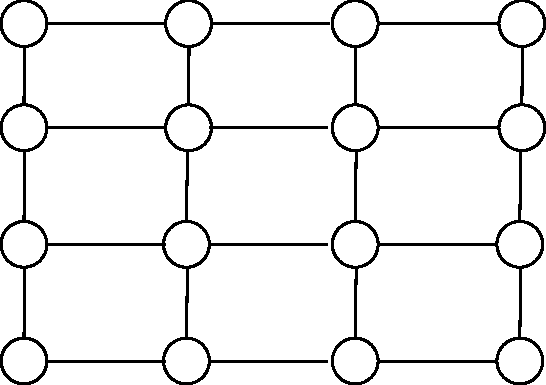
\includegraphics[width=0.25\textwidth]{fig/ising_1.pdf}}
\newline Recall the Ising model from a few lectures ago, a grid of nodes connected horizontally and vertically to adjacent nodes on 4 sides (or 3 on the edges and 2 on the corners).  Things in which we may be interested include the marginal distributions $p(y_{ij}=1)$ and the partition function.  Unlike for a tree structure, direct computation using loopy belief propagation may not converge well for this graph with cycles, so we will look for a different method.
\item Gaussian Mixture Model \\
\centerline{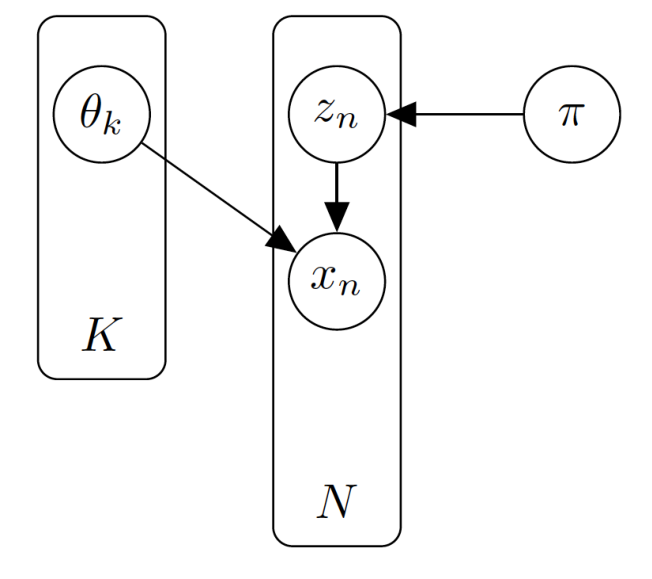
\includegraphics[width=0.25\textwidth]{fig/gmm.pdf}}
\begin{align*}
\pi & \sim dir(\alpha) \\
\Theta_k &= (\mu_k, \Sigma_k) \\
Z_n &\sim \pi \\
X_n | (Z_n, \Theta) &= N (\mu_k, \Sigma_k)
\end{align*}
Recall the Gaussian Mixture Model from last lecture, an unsupervised learning method that attempts to categorize data points into clusters.  This is nearly the same graphical model as Naive Bayes classification, except that the classes are not observed, but rather inferred.  Again, computation of $p(x_n)$ is rather difficult because $z_n$ are not observed.  Therefore, one must find a method that infers the $z_n$ in order to infer $p(x_n)$.
\end{itemize}

\subsection{Variational Idea}
\centerline{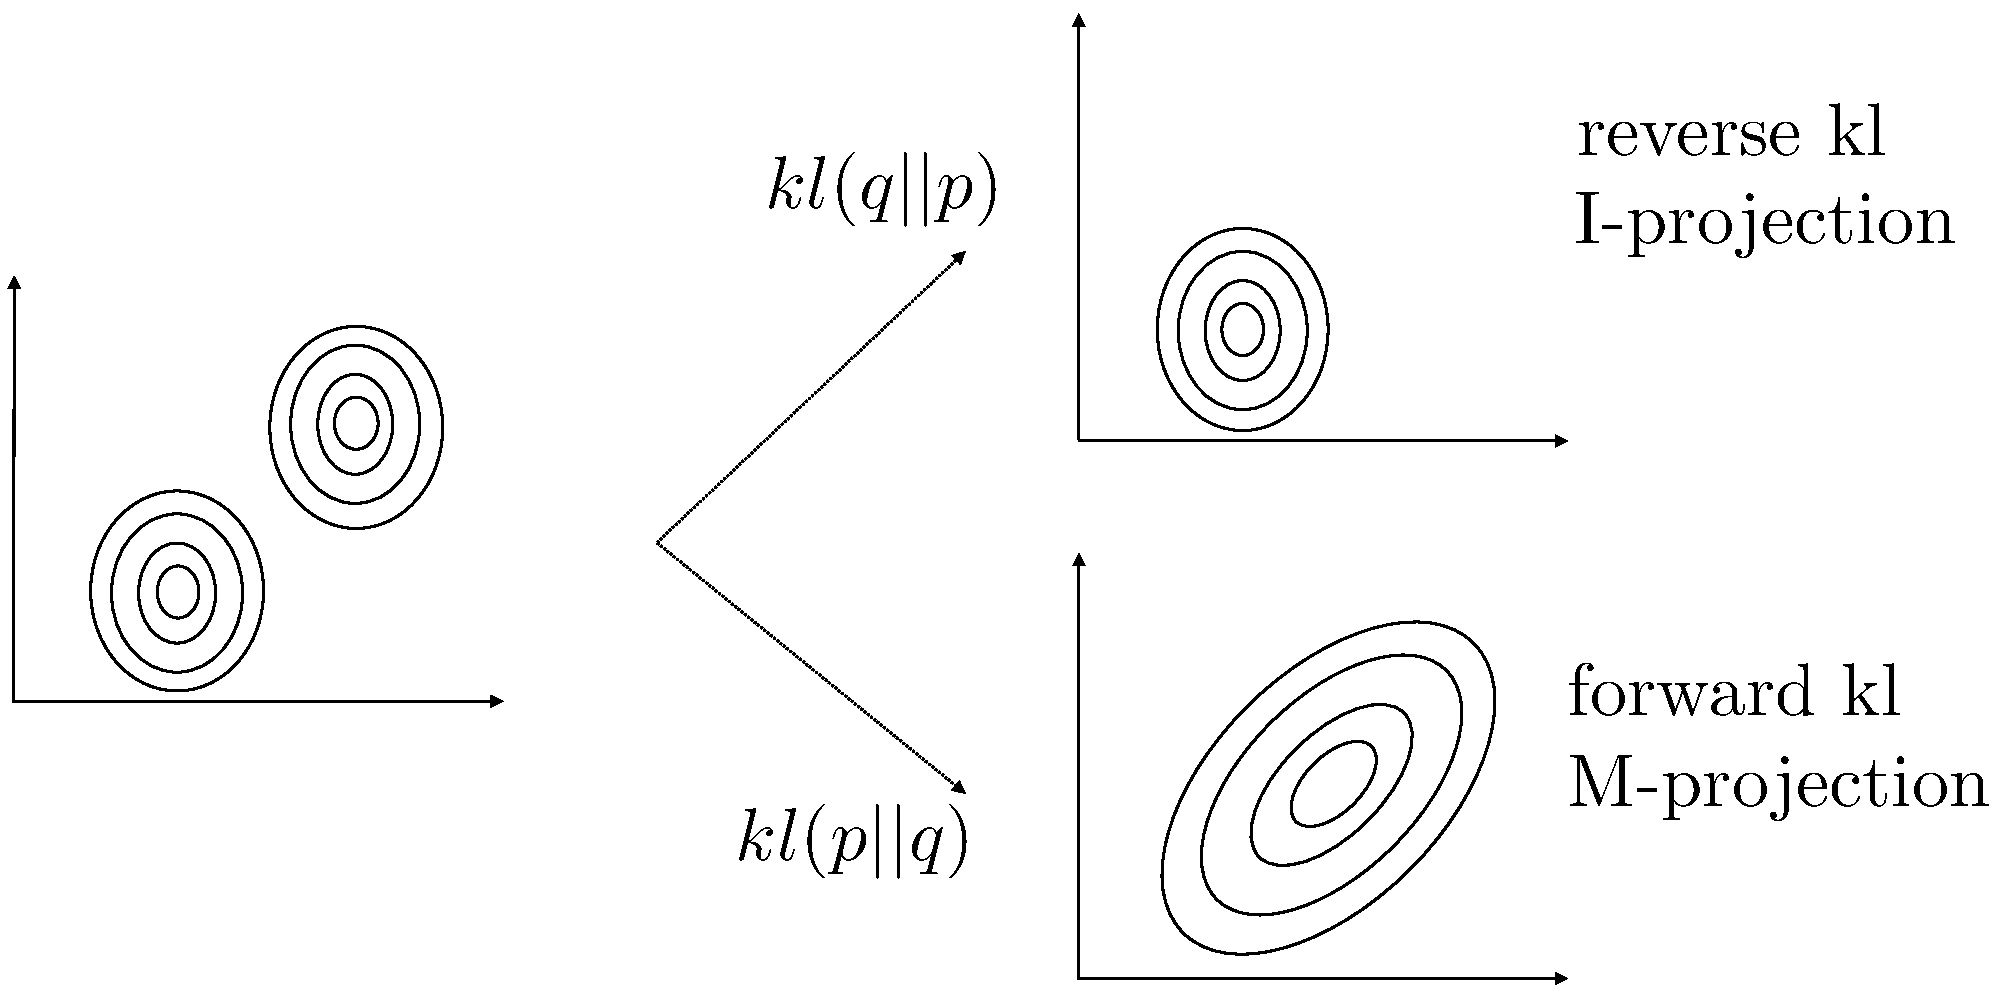
\includegraphics[width=0.75\textwidth]{fig/v_ideas.pdf}}
\begin{align*}
min_q d(p,q) &= KL(q \| p) \\
&= \int q(z) log \frac{q(z)}{p(z|D)}
\end{align*}
In trying find the gap function $d(p,q)$ that measures our gap from p to q, one good choice is the KL divergence, but because it is asymmetric, we essentially have 2 options, both of which lead to valid methods:
\begin{itemize}
\item $KL(q \| p)$ 
\newline The reverse KL, I-projection 
\item $KL(p \| q)$
\newline The forward KL, M-projection
\end{itemize}
The forward KL method is also known as the Expectation Propagation (EP) method.

\subsection{Relationship to EM}
Recall the Expectation-Maximization (EM) method from last lecture.  Much of the mathematics we will use resembles that which we have already studied.
\begin{align*}
\log p(D) &= \log \int_{z} p(D,z) dz \tag{D is the observed data set} \\
&= \log \int_{z} q(z) p(D,z)/q(z) dz \\
&= \log E_{z \sim q} \left[ \frac{p(D,z)}{q(D)}\right]\\
&\geq E_{z \sim q} \left[\log \frac{p(D,z)}{q(D)}\right] \tag{the lower bound, by Jensen's inequality}
\end{align*}
\begin{align*}
\log p(D) - E_q \log \frac{p(D,z)}{q(z)} &= E_q \left[\log p(D) - \log \frac{p(D,z)}{q(z)}\right] \\
&= E_q \left[\log \frac{q(z)}{p(z|D)} \right] \\
&= KL(q \| p)
\end{align*}
One more remaining issue is that
$$p(z|D) = \frac{p(z, D)}{p(D)}$$
\newline where $p(D)$ is generally very difficult to compute and the main reason why computing $p$ exactly becomes an intractable problem.  However, for the purposes of finding $q$, we can ignore $p(D)$ as just a constant, since it is independent of $z$.  Thus,
\begin{align*}
    \min_q KL(q \| p) = \min_q E \left[\log \frac{q(z)}{p(z, D)} \right]
\end{align*}
\subsection*{Comparison to EM}
\begin{itemize}
\item In variational inference, we have coordinate ascent just like in EM, except we try to optimize a lower bound.
\item In variational inference, we pick $q$ from the EASY set. As a result, we don't have to select point estimates, but rather we can use entire distributions.
\item This is very useful in Bayesian setups.
\item We can also combine this with EM and sampling to obtain more sophisticated techniques as well.
\end{itemize}

\subsection{Mean Field}
\centerline{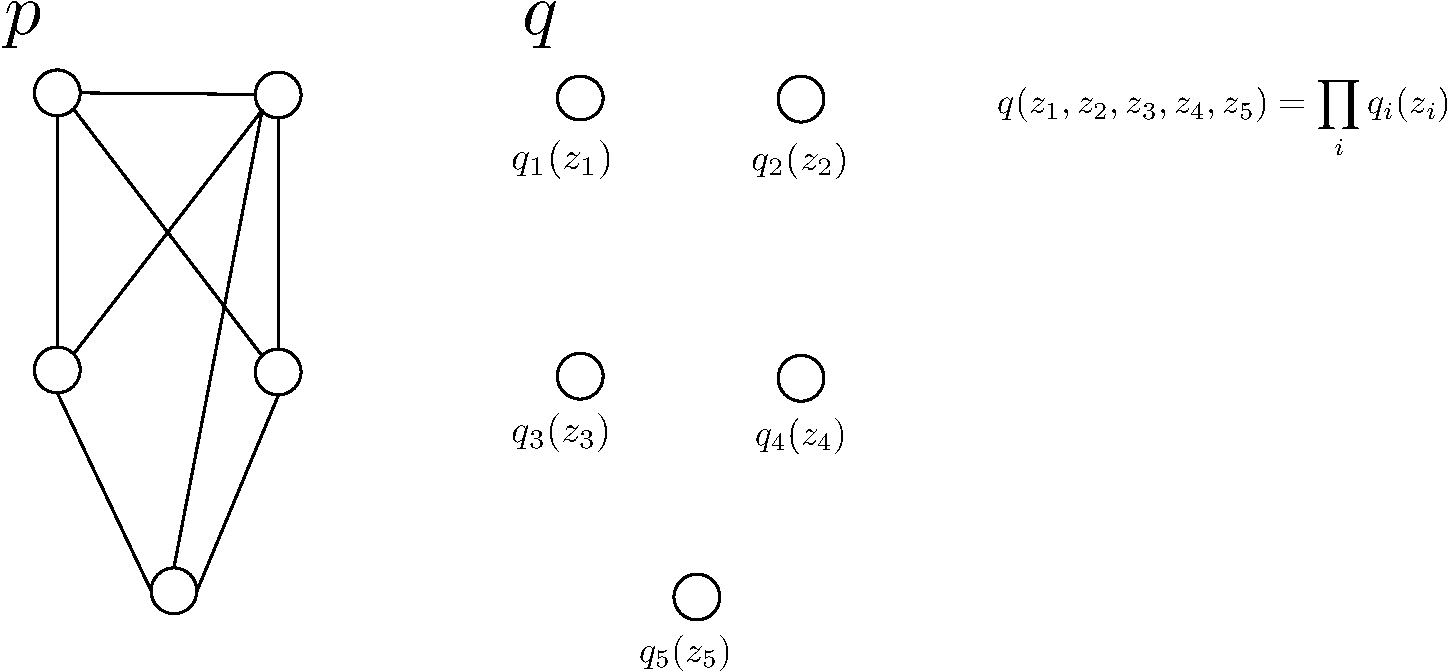
\includegraphics[width=0.75\textwidth]{fig/mean_field.pdf}}
This is an algorithm that optimizes one particular $q_i$, via an expectation over the adjacent variables, while fixing all of the other $q$ and then iterates this procedure over all of the $q$.  It proceeds as follows:
\begin{itemize}
\item We assume we have all $q$ except $q_i$.
\item Select $q(z) = \prod q_i (z_i)$ from our EASY set.
\item Recall that the goal is to reduce the gap $min_q KL(q\|p)$.  We do this by fitting each $q_i$ as
$$q_{i}^* \leftarrow argmin_q KL(q\|p)$$
where
\begin{align*}
argmin_q KL(q\|p) &= argmin_{q_i} -H(q_i)-E_q \log(p(z)) \\
& = argmin_{q_i} -H(q_i)-\int_z (\prod_i q_i (z_i))\log p(z) + other (j\neq i) \tag{q(z)=$\prod q_i(z_i)$} \\
&= argmin_{q_i} -H(q_i)-\int_{z_i} q_i(z_i) \int_{z_j: j\neq i} \prod_{j \neq i} q_i(z_i)\log p(z) + ... \\
&= argmin_{q_i} -H(q_i) - \int_{z_i} q_i(z_i) \log f_i \tag{$\log f_i= E_{q_i}[\log p(z)]$} \\
&= argmin_{q_i} KL(q_i \| f_i) \tag{$f_i$ is not distribution , but still OK}\\
q_i\propto exp\{E_{-q_i}(log(p(z)))\}
\end{align*}
\end{itemize}

Note that $E_{-q_i}$ denotes an expectation taken over all the variables except $z_i$.  

\subsection{Ising Model}
\centerline{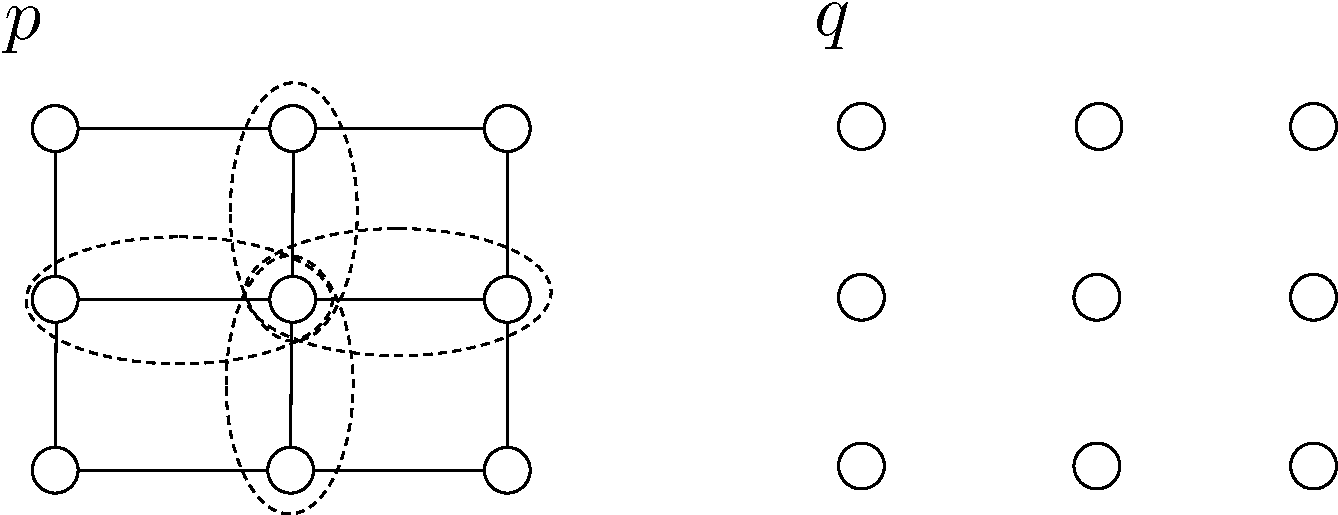
\includegraphics[width=0.75\textwidth]{fig/mean_field_ising.pdf}}
We now apply Mean Field Variational Inference to the Ising Model.  Note that $\theta_{v_i}$ denotes the log-potential of vertex $i$ while $\theta_{E_{i-n}}$ denotes the log-potential of the edge from vertex $i$ to vertex $n$.  We compute $q_i$ as an expectation over the 4 neighboring nodes, the Markov blanket.  This is then
\begin{align*}
q_i & \propto exp[E_{qi} \log p(z)] \\
p(z) & \propto exp[\theta_v^T z + z^T \theta_E z] \\
\log q_i(x_i) &\propto E_{-q_i} [\log p(z)] \\
&= E_{-q_i} [\theta_v^T z + z^T \theta_E z] \\
&= E_{-q_i} [z_i \theta_{v_i} + \Sigma_n \theta_{E_{i-n}} Z_i Z_n] \\
&= Z_i \theta_{v_i} + \Sigma_{n \in neighbor} \theta_{E_{i-n}} Z_i E_{q_n}[Z_n]\\
&= Z_i \theta_{v_i} + \Sigma_n \theta_{E_{i-n}} Z_i q_n(1)
\end{align*}
Therefore $$q_i \propto exp[Z_i \theta_{v_i} + \Sigma_n \theta_{E_{i-n}} Z_i q_n(1)]$$
We can then repeat this procedure over all nodes to update the entire graph.  Then we can repeat that over several epochs until we find good convergence of $q$.  

\end{document}